\documentclass{article}

\newcommand{\svninfo}{$ $Rev$ $, $ $Date$ $}
\pagestyle{myheadings}
\markboth{\svninfo}{\svninfo}

\usepackage{graphicx}
%\usepackage{pstricks}
\usepackage{xspace}
\usepackage{amsmath}
\usepackage{natbib}
\usepackage{todo}
\usepackage[british]{babel}
\usepackage[left=1in,right=1in,top=1in,bottom=1in]{geometry}

\newcommand{\figref}[1]{\textbf{(#1)}}
\newcommand{\EE}{\ensuremath{E_\mathrm{E}}\xspace}
\newcommand{\EA}{\ensuremath{E_\mathrm{A}}\xspace}
\newcommand{\ED}{\ensuremath{E_\mathrm{D}}\xspace}
\newcommand{\Ed}{\ensuremath{E_\mathrm{d}}\xspace}
\newcommand{\p}{\vec{p}}
\newcommand{\q}{\vec{q}}


\title{Deformation of an elastic hemisphere}
\author{David Sterratt}

\begin{document}
\maketitle
\thispagestyle{myheadings}

As a test of the retinal folding program, I would like to construct a
test case in which an object of known geometry is flattened. The
algorithm will then be used to morph this object back to its original
shape, and the difference in the locations of landmarks on the
original and reconstructed objects will be a measure of the error in
the reconstruction process.

\begin{figure}[h]
  \centering
  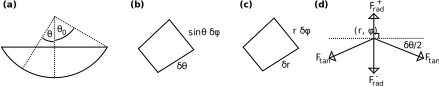
\includegraphics{hemisphere}
  \caption{\figref{a} Cross-section of a sphere curtailed at an angle
    $\theta_0$ from its axis. \figref{b} Rectangle on intact
    sphere. \figref{c} Rectangle on flattened sphere. \figref{d}
    Forces acting on a point on the lattice.}
  \label{deformation:fig:hemisphere}
\end{figure}

A simple object to start on is a curtailed sphere of unit radius
constructed from an elastic material
(Figure~\ref{deformation:fig:hemisphere}a). The angle at which the
sphere is curtailed is $\theta_0$ from the principal axis.

Now consider that this shape has been squished flat between two rigid
surfaces. Assuming that axial symmetry is maintained, so that there is
a mapping $f$ of latitude $\theta$ (measured from the base of the
curtailed sphere) onto radial distance $r$.  The aim is to compute
this mapping $f$.

In order to predict the deformation, consider segmenting the sphere
into small regions bounded by the lines of latitude at $\theta$ and
$\theta+\delta\theta$ and the lines of longitude $\phi$ and
$\phi+\delta\phi$. The dimensions of each small rectangle created by
this lattice are $\delta\theta$ by $\sin\theta\;\delta\phi$
(Figure~\ref{deformation:fig:hemisphere}b).

The ``spring constant'' of a rectangle in the direction of one of its
axes should be proportional to the length of the side perpendicular to
the axis and inversely proportional to the side parallel to the
axis. Thus the radial and tangential spring constants of the rectangle are
\begin{equation}
\label{deformation:eq:1}
  k_\mathrm{rad} = \frac{\sin\theta\;\delta\phi}{\delta\theta}
  \quad\mbox{and}\quad
  k_\mathrm{tan} = \frac{\delta\theta}{\sin\theta\;\delta\phi}
\end{equation}

In the flattened object, each rectangle is mapped to a new rectangle
with dimensions $\delta r$ by $r\delta\phi$
(Figure~\ref{deformation:fig:hemisphere}c). The forces acting at every
point $(r, \phi)$ in the flattened object are assumed to be in
equilibrium (Figure~\ref{deformation:fig:hemisphere}d). Due to axial
symmetry, the net force in the tangential direction is zero. The
forces in the radial direction are the outward radial force,
$F^+_\mathrm{rad}$, the inward radial force, $F^-_\mathrm{rad}$ and
two components of the tangential forces in the radial direction. The
equilibrium equation therefore reads:
\begin{displaymath}
  F^+_\mathrm{rad} - F^-_\mathrm{rad} -
  2\frac{\delta\phi}{2}F_\mathrm{tan} = 0
\end{displaymath}
On the assumption of linear elasticity, each force is the product of
the change in length of side of the rectangle and the spring constant,
so the equilibrium equation becomes:
\begin{displaymath}
  k_\mathrm{rad}(f(\theta+\delta\theta)-f(\theta) - \delta\theta) 
  - k_\mathrm{rad}(f(\theta)- f(\theta-\delta\theta) - \delta\theta) 
 - \delta\phi  k_\mathrm{tan} (f(\theta) \delta\phi - \sin\theta
 \delta\phi) = 0
\end{displaymath}
Substituting in the spring constants from
equation~(\ref{deformation:eq:1}), and using the approximation
\begin{displaymath}
f(\theta+\delta\theta)-2f(\theta)+f(\theta-\delta\theta)\approx
\frac{\mathrm{d}^2r}{\mathrm{d}\theta^2}\delta\theta^2
\end{displaymath}
where $r=f(\theta)$ we obtain:
\begin{displaymath}
  \sin^2\theta \frac{\mathrm{d}^2r}{\mathrm{d}\theta^2}
  - (r - \sin\theta)=0
\end{displaymath}
It would be great if we could solve this analytically!

I've tried substituting $u=\sin\theta$, which (I think) gives:
\begin{displaymath}
  u^2(1-u^2) \frac{\mathrm{d}^2r}{\mathrm{d}u^2} 
  -u^3 \frac{\mathrm{d}r}{\mathrm{d}u} 
  -r + u = 0
\end{displaymath}
but I don't know if this helps much.

\bibliographystyle{natbib}
\bibliography{mystrings,my}

\end{document}

%%% Local Variables: 
%%% TeX-PDF-mode: t
%%% End: 

% LocalWords:  mystrings
